%\subsection{One processing step in PROV-N notation}
%
%\TODO{Put the very simple example here}
%See \url{https://volute.g-vo.org/svn/trunk/projects/dm/provenance/description/prov-example-incl-prototypes.txt}
%and \url{https://volute.g-vo.org/svn/trunk/projects/dm/provenance/description/prov-example-w3c.txt}

This section presents some general guidelines for applying the data model and
%This section presents some 
specific use cases for which the provenance data model helps to solve certain tasks. Details on specific implementions of the provenance data model are provided in a separate document, the ProvenanceDM Implementation Note \citep{std:ProvenanceImplementationNote}.


\subsection{How to use the data model}
\TODO{KR: I think this is a good place for this section. Do we still want to have this section or is everything covered with the new section on entitydescription-serialisation?}
\begin{itemize}
\item identify entities in your project, i.e. the things you deal with
\item identify activities (processes) in your project
\item identify reponsible agents (persons and organizations)
\item find the relations between them
\item possibly disentangle entity properties and entityDescription properties: everything that you may know about an entity before its creation, belongs to the entityDescription; e.g. file format, dataProduct\_type, what kind of entity it is going to be (category)
\item ...
\end{itemize}

The IVOA Provenance data model has been developed along with its implementations into different projects. We gather here some tips to apply the model to a specific project.

\paragraph{Before using the model}. We noticed that the simple knowledge of what is provenance information is important for the development of all projects. Before using or not the Provenance data model and associated services, it is good practice to locate and collect information on activities, entities and agents, and be sure that this information is not lost along the way. For example, a script may use intermediate files (such as calibration files for observations) that may not be tracked by the system.


\paragraph{Use of the description side}. 
One may only use the core data model without the description classes if they are not needed for the project. In that case, it is recommended to include the attributes of the description classes into the main classes (Entity/Activity/Agent, and if needed Parameter). In the same way, when serializing the provenance information, the description classes can be merged to the main classes, which is needed to produce W3C compliant provenance files.

\paragraph{Identify entities, activities and agents}.
If inside the project, the different entities are already identified, as well as the activities producing them, then the description classes are probably of interest and will help to reduce the redundancy in the provenance information stored.

\paragraph{add project specific attributes to entities, activities and agents}.
We proposed generic attribute for the different classes, but there are probably project specific attributes that need to be added. What is important to define the project activities ? 



\subsection{voprov Python package}\label{sec:implementation_voprov}
The voprov Python package is derived from the voprov-package. It can load
data and serialize it. The voprov-package supports following features:
...
\TODO{Michele: Please add more explanations!}
%This code writes the serialisation examples which are given in Section~\ref{sec:serialisations}.

Example code and serializations are given in the Implementation Note \citep{std:ProvenanceImplementationNote}.


\subsubsection{Graphic formats}
\label{sec:graphic_formats}
The voprov python module can also provide provenance information in graphic formats: PNG, SVG and PDF.
In the above example, you have to add the following instructions in your python program:

\begin{verbatim}
    dot = prov_to_dot(provdoc, use_labels=True)
    dot.write_png('ex1.png')
    dot.write_svg('ex1.svg')
    dot.write_pdf('ex1.pdf')
\end{verbatim}

\begin{figure}
\centering
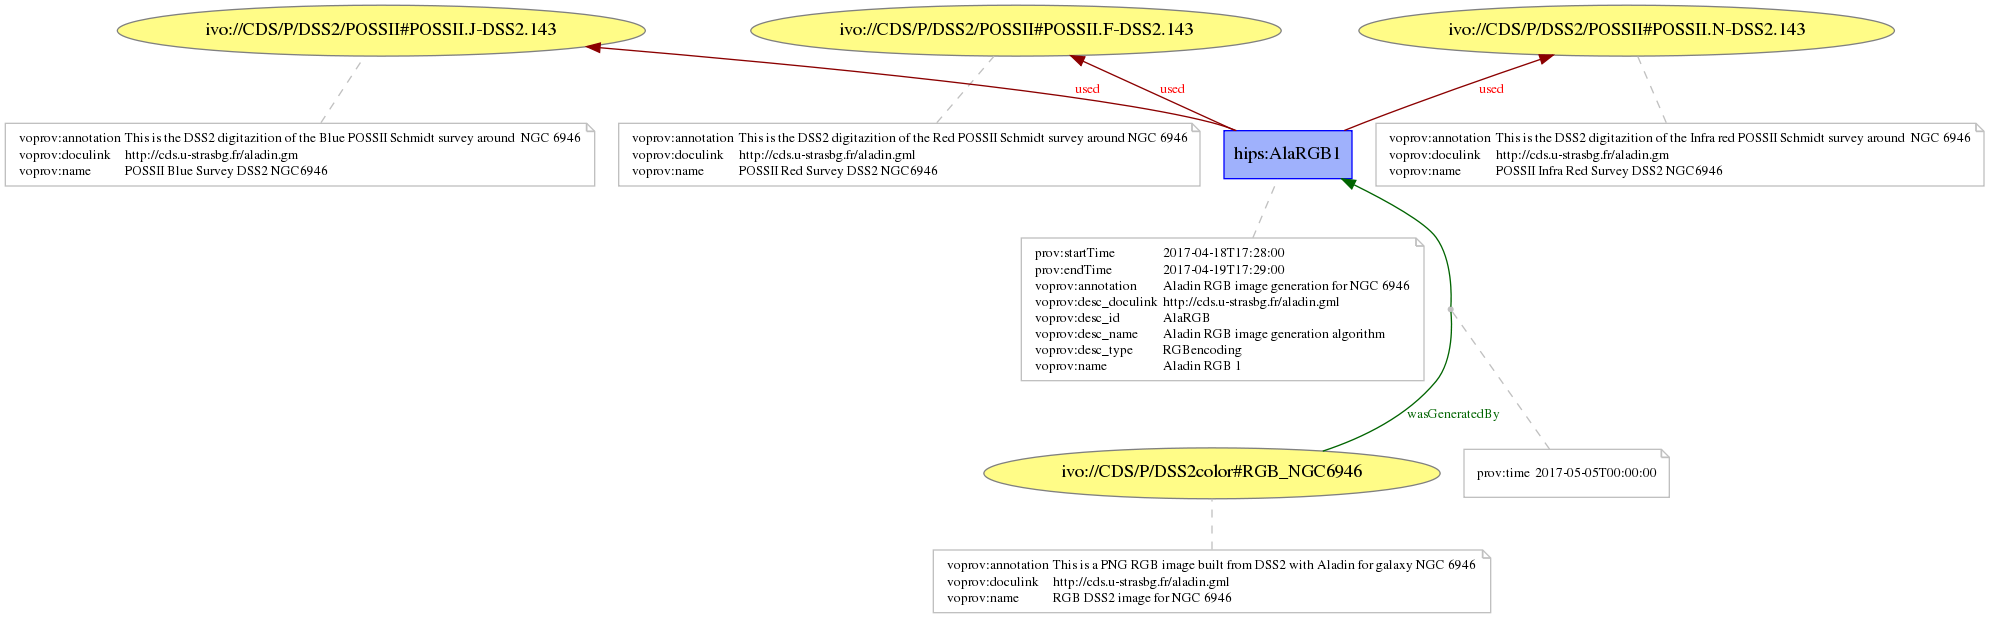
\includegraphics[width=0.9\textwidth]{access_ex1.png}
\caption{Example: png format@}
\label{fig:example}
\end{figure}



\subsection{Provenance of RAVE database tables (DR4)}
The RAVE survey (Radial Velocity Experiment) recorded spectra for about half a 
million stars. These spectra are processed in a number of steps until the 
derived properties are published in the RAVE data releases at http://www.rave-survey.org.
Providing provenance information for the data, from which spectrum and fibre the
data was coming from and which steps were involved in processing the data, can help scientists
to understand the data and their restrictions and judge their quality.
It would also be useful to be able to compare if, how and why the derived data 
for some stars have changed between different releases.
Provenance information for some major steps of RAVE DR4 was loaded in 
W3C-compatible PROV-N notation and uploaded to the provenance store at 
https://provenance.ecs.soton.ac.uk/store/documents/84064/. This allows to view 
graphs of the workflow by visualising only the main entities, activities and agents 
with their relations. It shows that the provenance concepts explained in this draft 
can be applied directly to data obtained from astronomical observations.

We also tested a Django implementation of the classes in this document along with provenance data stored in an SQLite database. This allows to quickly setup a provenance web service
which gives the possibility to view all instances of a class or details for a single object, 
extract provenance information for single entities (backwards in time) and 
visualise the provenance information. 
More details about this are available in the implementation notes \citep{std:ProvenanceImplementationNote}.




\subsection{Provenance for CTA}

The Cherenkov Telescope Array (CTA) is the next generation ground-based very high energy gamma-ray instrument. It will provide a deep insight into the non-thermal high-energy universe. Contrary to previous Cherenkov experiments, it will serve as an open observatory providing data to a wide astrophysics community, with the requirement to propose self-described data products to users that may be unaware of the Cherenkov astronomy specificities. The proposed structure of the metadata is presented in Figure~\ref{fig:cta_dm}.

\begin{figure}
\centering
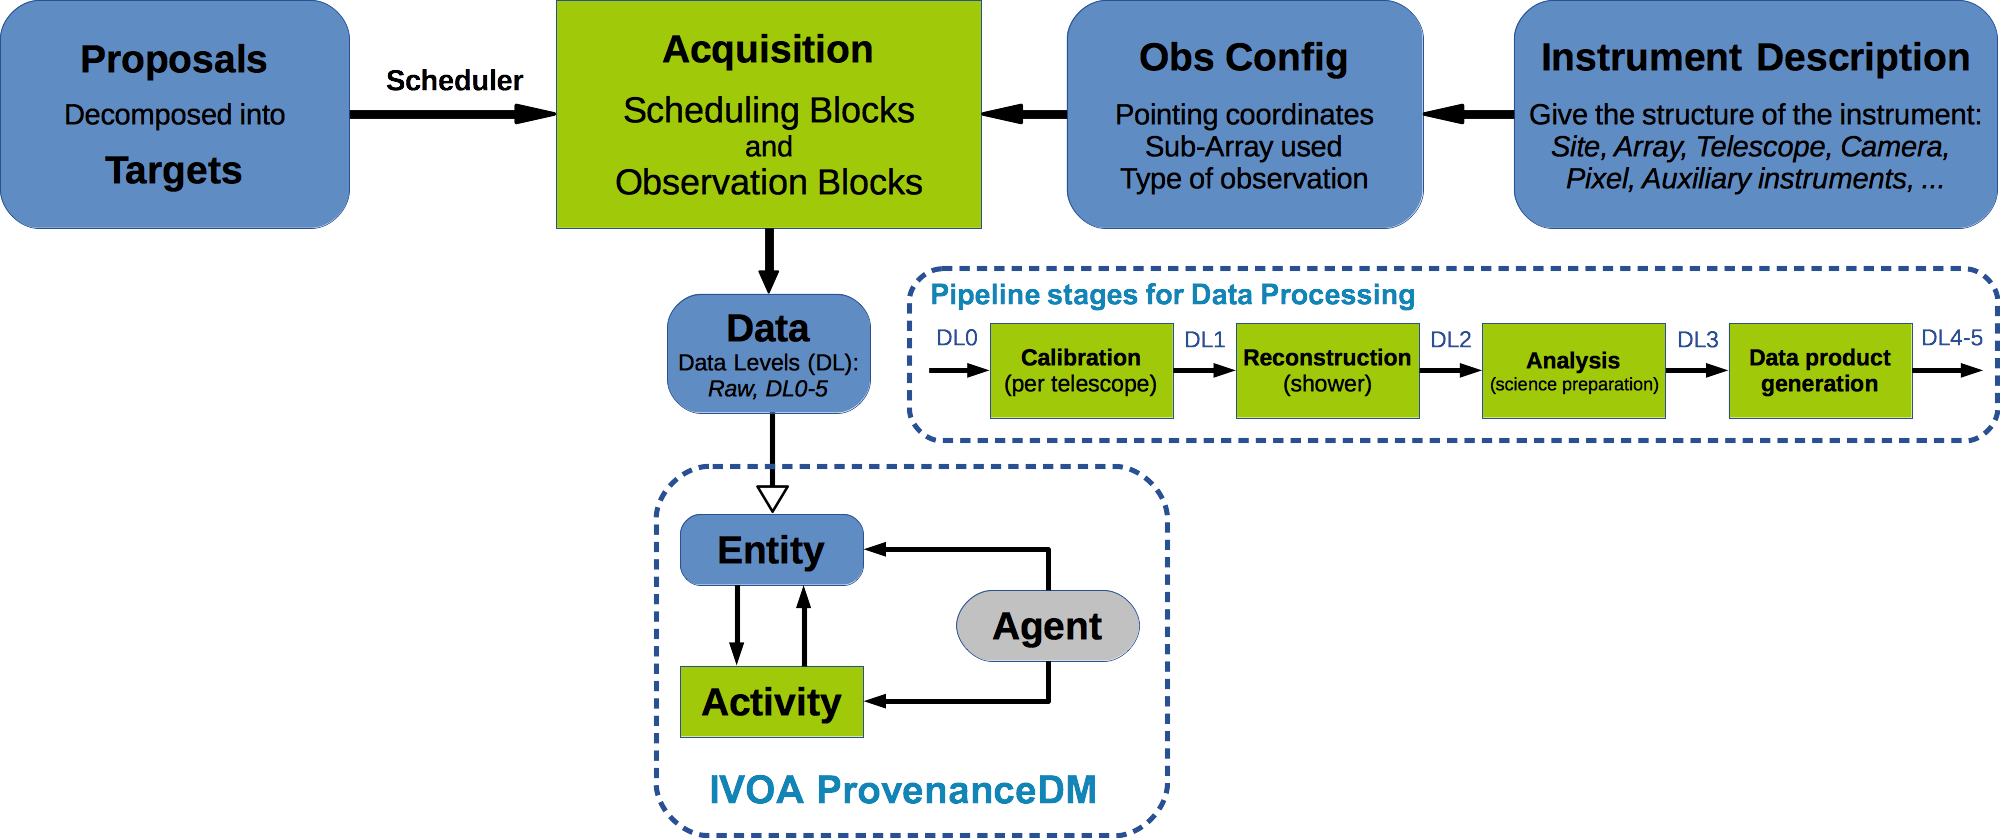
\includegraphics[width=\textwidth]{CTA_DM_high_level.png}
\caption{CTA high level data model structure with Pipeline stages and connection to IVOA ProvenanceDM.}
\label{fig:cta_dm}
\end{figure}

Cherenkov telescopes indirectly detect gamma-rays by observing the flashes of Cherenkov light emitted by particle cascades initiated when the gamma-rays interact with nuclei in the atmosphere. The main difficulty  is that charged cosmic rays also produce such cascades in the atmosphere, which represent an enormous background compared to genuine gamma-ray-induced cascades. Monte Carlo simulations of the shower development and Cherenkov light emission and detection, corresponding to many different observing conditions, are used to model the response of the detectors.  With an array of such detectors the shower is observed  from several points and, working backwards, one can figure out the origin, energy and time of the incident particle. The main stages of the CTA Pipeline are presented inside Figure~\ref{fig:cta_dm}. Because of this complexity in the detection process, provenance information of data products is necessary to the user to perform a correct scientific analysis.

Provenance concepts are relevant for different aspects of CTA :
\begin{itemize}
\item Data diffusion: the diffused data products have to contain all the relevant context information with the assumptions made as well as a description of the methods and algorithms used during the data processing.
\item Pipeline: the CTA Observatory must ensure that data processing is traceable and reproducible.
\item Instrument Configuration: the characteristics of the instrument at a given time have to be available and traceable (hardware changes, measurements of e.g. a reflectivity curve of a mirror, ...)
\end{itemize}

We tested the tracking of Provenance information using the Python prov package inside OPUS\footnote{\url{https://github.com/ParisAstronomicalDataCentre/OPUS}} (Observatoire de Paris UWS System), a job control system developed at PADC (Paris Astronomical Data Centre). This system has been used to run CTA analysis tools and provides a description of the Provenance in the PROV-XML or PROV-JSON serialisations, as well as a graph visualization (see Figure~\ref{fig:cta_prov}).

\begin{figure}
\centering
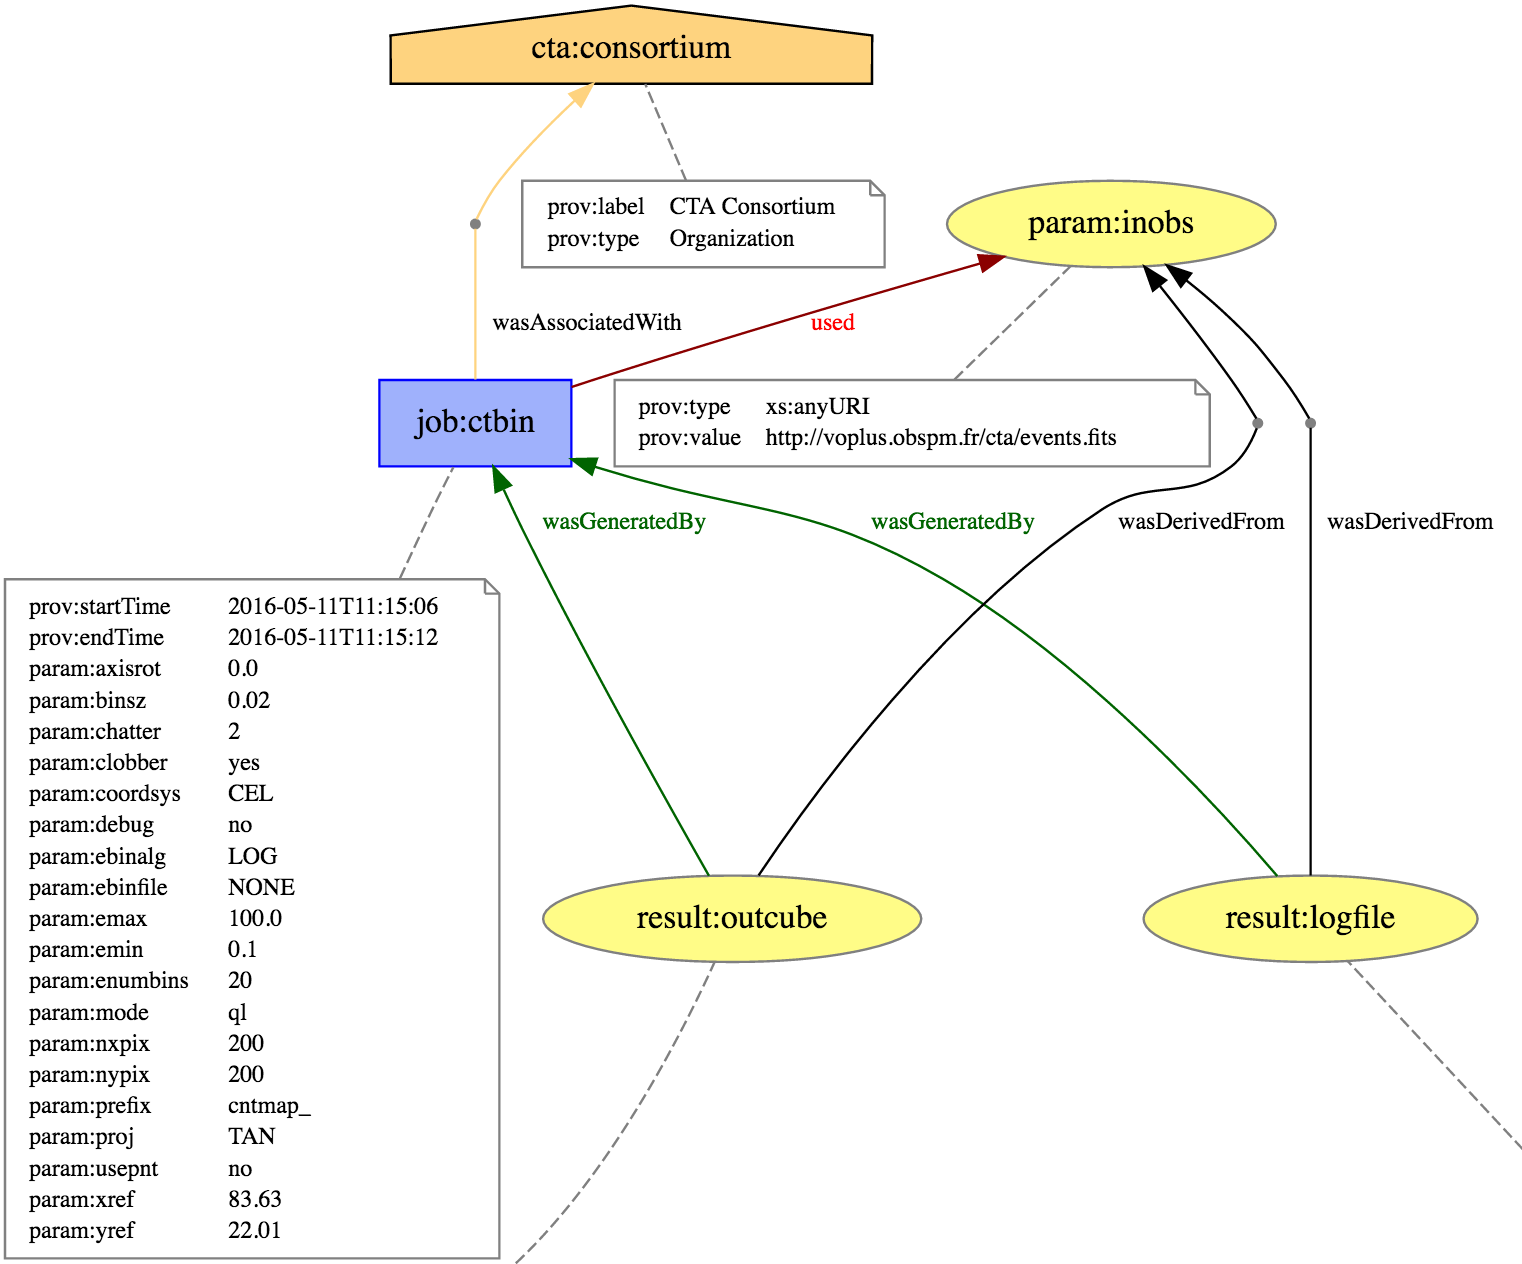
\includegraphics[width=0.8\textwidth]{CTA_prov.png}
\caption{Provenance description of a CTA analysis step.}
\label{fig:cta_prov}
\end{figure}


\subsection{POLLUX database}

POLLUX is a stellar spectra database proposing access to high resolution synthetic spectra computed using the best available models of atmosphere (CMFGEN, ATLAS and MARCS), performant spectral synthesis codes (CMF\_FLUX,SYNSPEC and TURBOSPECTRUM) and atomic linelists from VALD database and specific molecular linelists for cool stars. 

Currently the provenance information is given to the astronomer in the header of the spectra files (depending on the format: FITS, ascii, xml, votables, ...) but in a non normalized description format. 

The implementation of the provenance concepts in a standardized format allows users on one hand to benefit from tools to create, visualize and transform in another format the description of the provenance of these spectra and on a second hand to select data depending on provenance criteria.

\begin{figure}
\centering
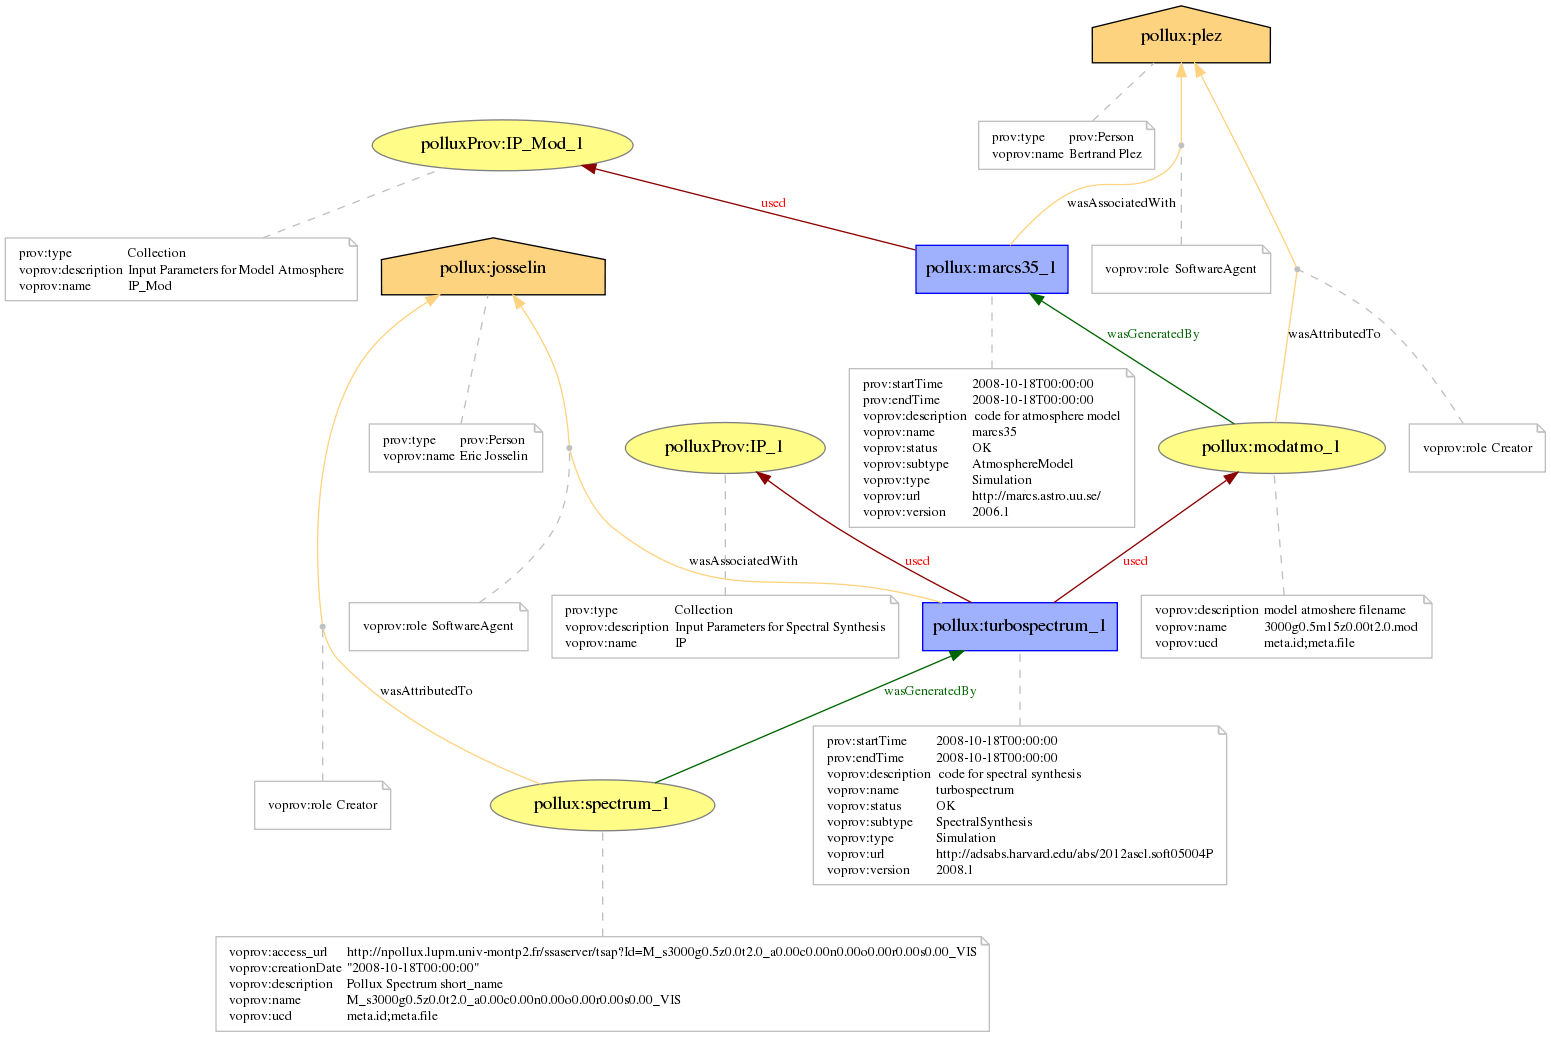
\includegraphics[width=0.9\textwidth]{usecase_Pollux_example1.png}
\caption{Pollux Example 1}
\label{fig:pollux}
\end{figure}

\subsection{HiPS use case}
HiPS is a new all sky organization of pixel data. It is based on HealPix tesselation of the sky on equal area cells (pixels) for a given HealPix order gathered in tiles. Adaptative resolution is achieved by a hierarchy of tiles at increasing order. Sorting and organization is based on a tree of including directories each of those associated with a tile. HiPS specification has entered the IVOA recommendation process and is becoming an interoperability standard.
In the processing chain, HiPS can be seen as a kind of ``legacy level'' for observational data.

An HiPS dataset can be generated either by Aladin in ``hipsgen'' mode or by other softwares.  The processing distinguishes 3 main different methods for estimating cell values: FIRST or NEAREST neighbour, Mean or Median of the neigbouring pixels. Up to 50 parameters can help to tune the processing, among which can be found the higher resolution HealPix order, sky background value to be substracted, border width or mask to apply to original images to avoid including bad area in the computing, etc.

An example of provenance metadata for a HiPS collection generated from a collection of SERC Schmidt plates scanned by CAI (Observatoire de Paris) with the MAMA facility and serialized in PROV-N format is given at 
\url{https://volute.g-vo.org/svn/trunk/projects/dm/provenance/example/HiPS-prov-provn.txt}, the corresponding votable-format is available at \url{https://volute.g-vo.org/svn/trunk/projects/dm/provenance/example/HiPS-prov-vot.xml}.

Here is an extract of the PROV-N serialization:

\begin{verbatim}
Entity
( ivo://CDS/P/MAMA/ESO-R, 
[
prov:label = "ESO-R MAMA HIPS at CDS",
prov:annotation = "This is the HiPS version of ESO Schmidt survey digitized by Mama and processed by CDS",
hips:HiPS_properties = "http://cds.u-strasbg.fr/hips/p/mama/eso-r/properties.txt",
voprov:access_reference = "http://CDS/P/MAMA/ESO-R", // as defined in obscore 
voprov:doculink = "http://cds.u-strasbg.fr/hips/documentation.html#structure",
voprov:dataproduct_type = "voprov:hips_pixels",
voprov:level = 3
]
)

// Relationship
WasAttributedTo(ivo://CDS/P/MAMA/ESO-R, ivo://cds, prov:role = "voprov:creator")

Agent
(ivo://cds,
[
voprov:Name = "CDS",
voprov:contact = "question@astro.unistra.fr",
prov:type = "Organisation"
]
)
\end{verbatim}

% WasGeneratedBy(ivo://CDS/P/MAMA/ESO-R, EHG1, -)

% Activity
% (EHG1,
% [
% prov:label = "ESO HiPS generation 1",
% prov:startTime = "2016-07-18",
% prov:endTime = "2016-07-20",
% voprov:annotation = "This activity is final generation of HiPS for ESO Mama survey",
% voprov:activityDescription = "HipsgenM"
% ]
% )

% ActivityDescription 
% (HipsgenM,
% [
% prov:label = "HiPS Generation MEAN",
% prov:type = "HiPSgen",
% voprov:subtype = "HiPSgen_MEAN",
% voprov:doculink = "http://cds.u-strasbg.fr/HiPSGEN-Documentation"
% ]
% )
%\end{verbatim}


\subsection{Lightcurves use case}
TBD. See Provenance webpage in IVOA Twiki for now.
